% Editable native annotations around unchanged verified IDE photographs.
\par
\begin{figure}[htbp]
  \centering
  \sbox0{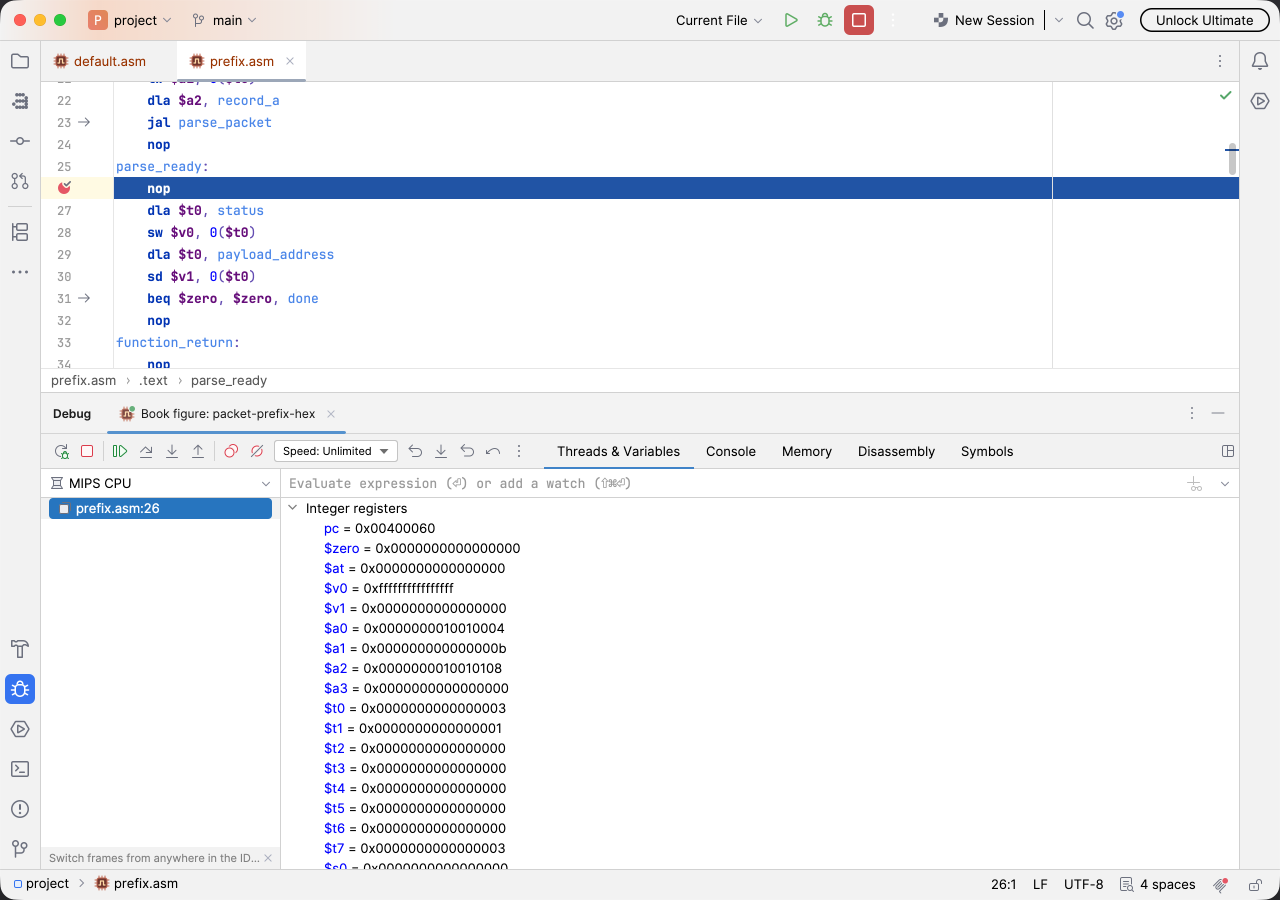
\includegraphics[artifact]{packages/013-binary-packet-parser/captures/f02-prefix/hex.png}}
  \sbox2{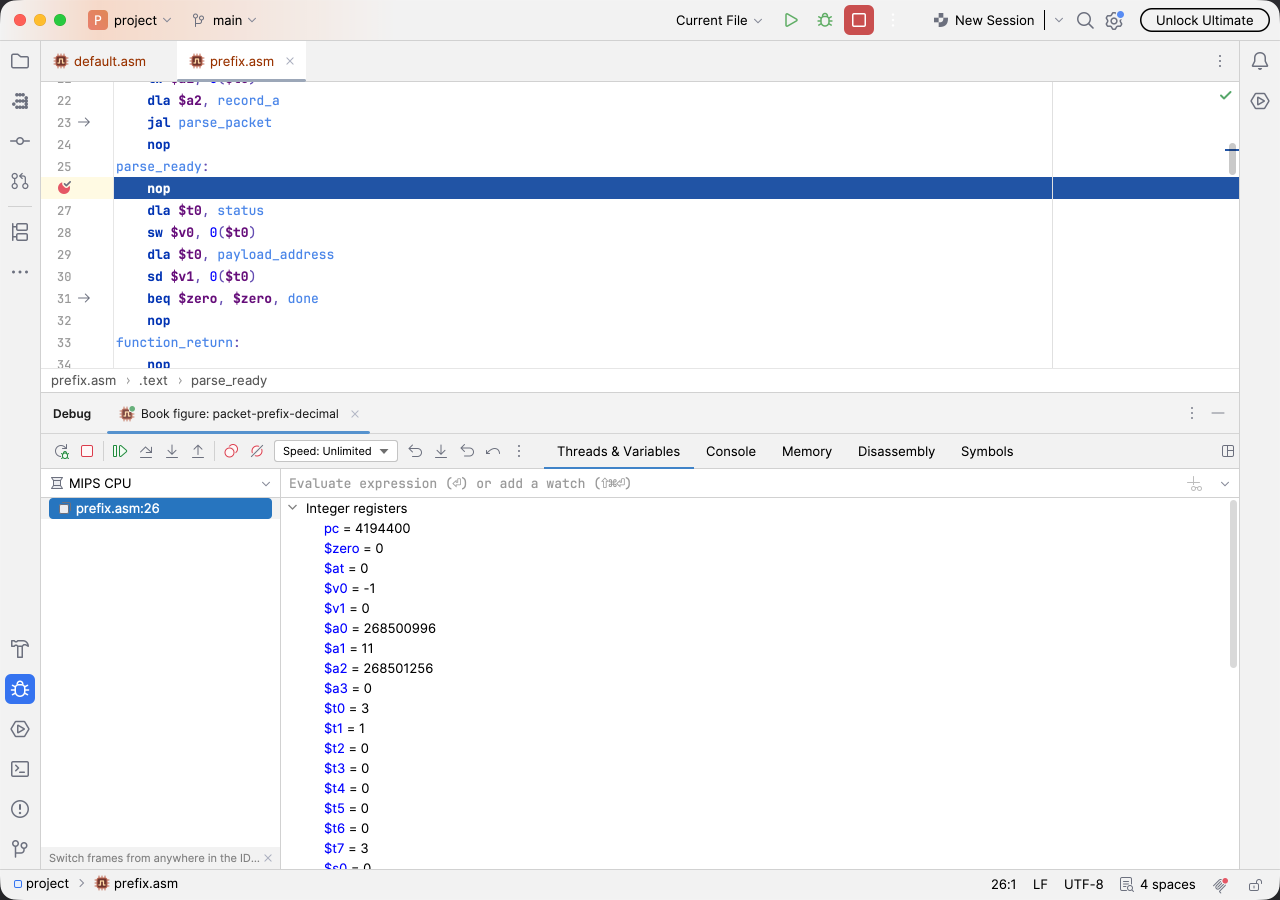
\includegraphics[artifact]{packages/013-binary-packet-parser/captures/f02-prefix/decimal.png}}
  \sbox4{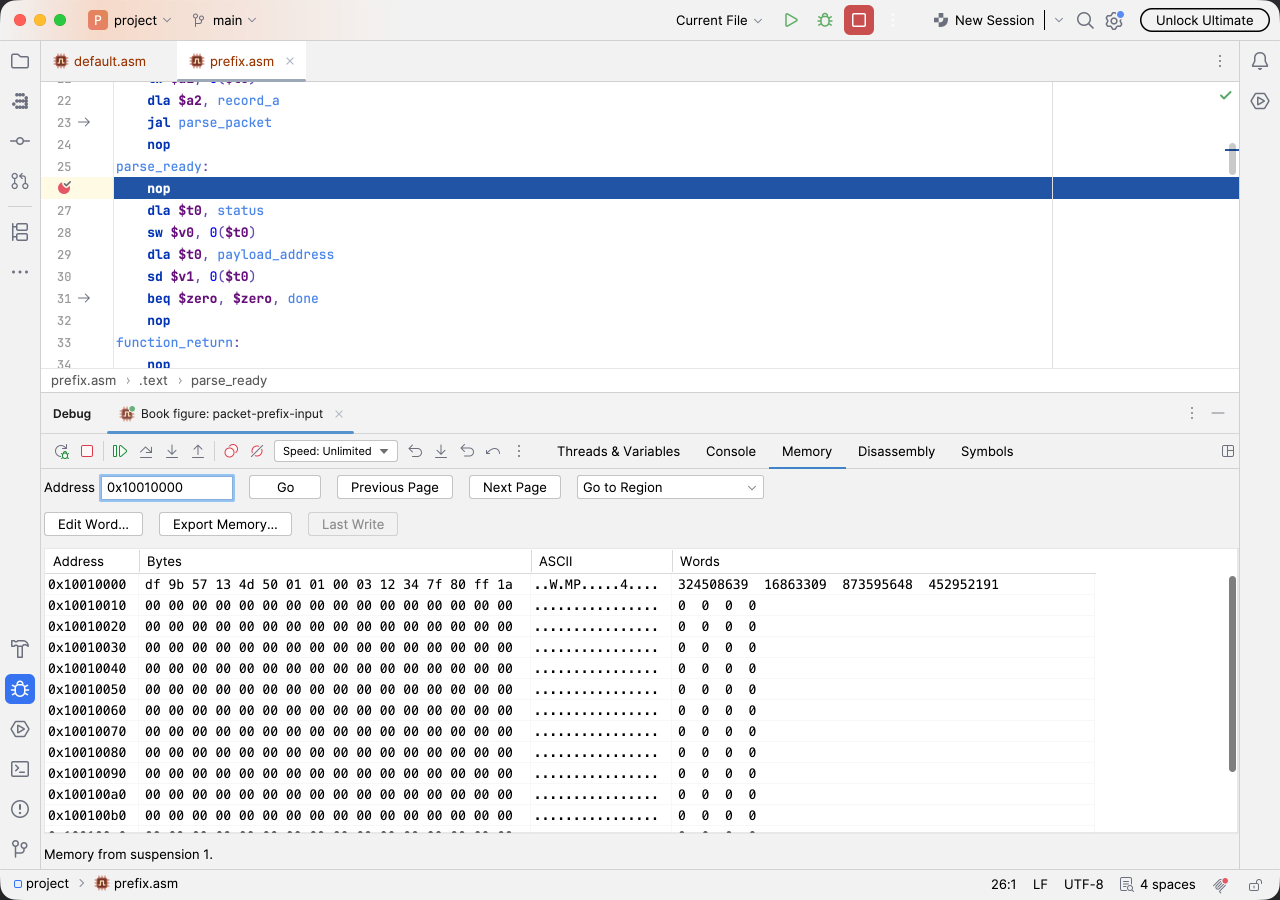
\includegraphics[artifact]{packages/013-binary-packet-parser/captures/f02-prefix/input.png}}
  \sbox6{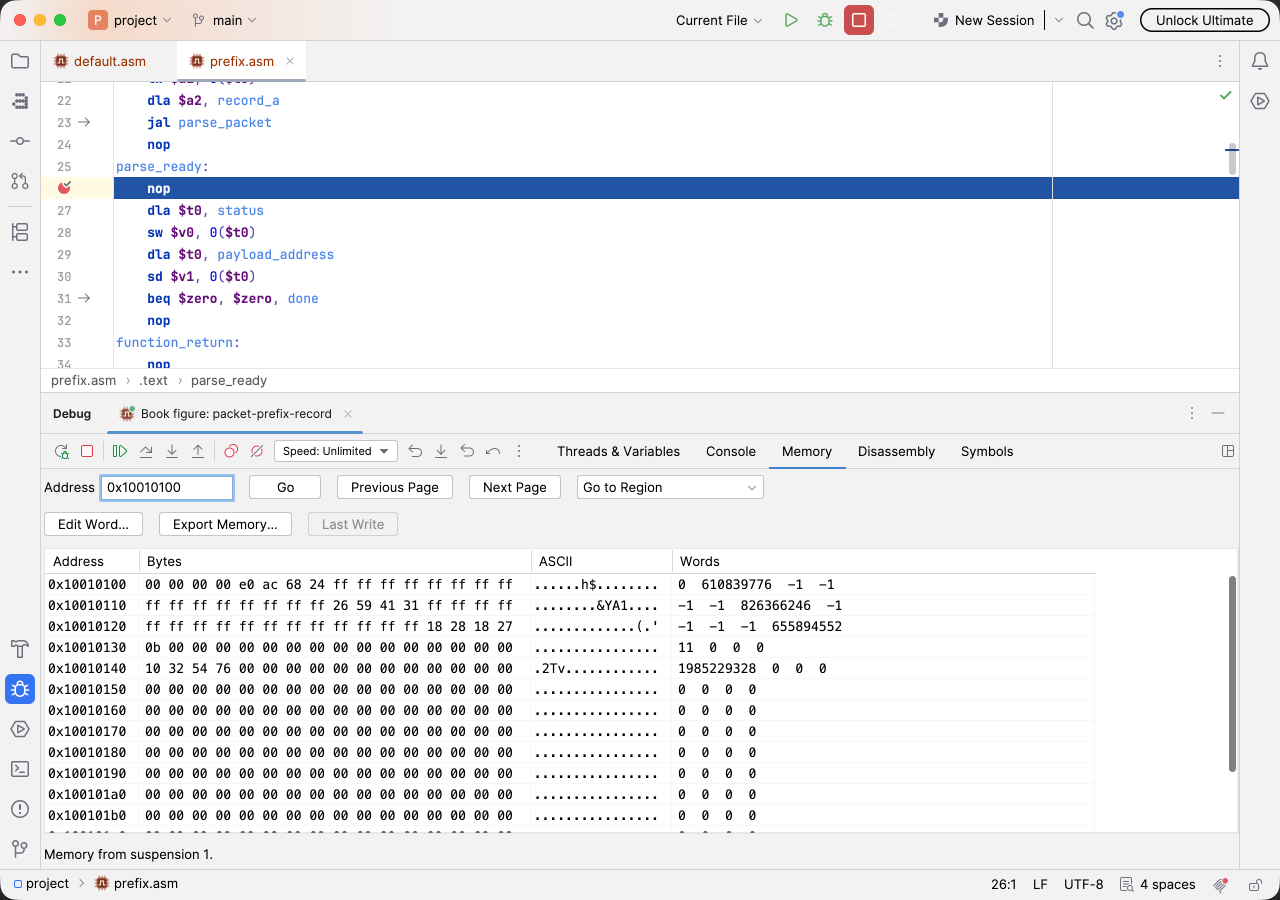
\includegraphics[artifact]{packages/013-binary-packet-parser/captures/f02-prefix/record.png}}
  \edef\MARSpacketprefixsourceLeft{\the\dimexpr0.036718750\wd0\relax}
  \edef\MARSpacketprefixsourceBottom{\the\dimexpr0.774444444\ht0\relax}
  \edef\MARSpacketprefixsourceRight{\the\dimexpr0.713281250\wd0\relax}
  \edef\MARSpacketprefixsourceTop{\the\dimexpr0.147777778\ht0\relax}
  \edef\MARSpacketprefixhexLeft{\the\dimexpr0.246093750\wd0\relax}
  \edef\MARSpacketprefixhexBottom{\the\dimexpr0.245555556\ht0\relax}
  \edef\MARSpacketprefixhexRight{\the\dimexpr0.553906250\wd0\relax}
  \edef\MARSpacketprefixhexTop{\the\dimexpr0.640000000\ht0\relax}
  \edef\MARSpacketprefixdecimalLeft{\the\dimexpr0.246093750\wd2\relax}
  \edef\MARSpacketprefixdecimalBottom{\the\dimexpr0.312222222\ht2\relax}
  \edef\MARSpacketprefixdecimalRight{\the\dimexpr0.553906250\wd2\relax}
  \edef\MARSpacketprefixdecimalTop{\the\dimexpr0.640000000\ht2\relax}
  \edef\MARSpacketprefixinputLeft{\the\dimexpr0.034375000\wd4\relax}
  \edef\MARSpacketprefixinputBottom{\the\dimexpr0.334444444\ht4\relax}
  \edef\MARSpacketprefixinputRight{\the\dimexpr0.584375000\wd4\relax}
  \edef\MARSpacketprefixinputTop{\the\dimexpr0.608888889\ht4\relax}
  \edef\MARSpacketprefixrecordLeft{\the\dimexpr0.034375000\wd6\relax}
  \edef\MARSpacketprefixrecordBottom{\the\dimexpr0.311111111\ht6\relax}
  \edef\MARSpacketprefixrecordRight{\the\dimexpr0.584375000\wd6\relax}
  \edef\MARSpacketprefixrecordTop{\the\dimexpr0.608888889\ht6\relax}
  \begin{tikzpicture}[alt={Five annotated details at parser return for an eleven-byte prefix of the unchanged valid packet. The available register is eleven; native signed status is minus one and the payload pointer is zero. The mapped checksum byte 0x1a is visible at input plus eleven, just beyond the logical prefix. All four record A words retain minus one.}]
    \node[anchor=north west,inner sep=0,font=\small\bfseries] (source-title) at (6mm,0) {Next instruction after return};
    \node[anchor=north west,inner sep=0] (source) at ([yshift=-1mm]source-title.south west) {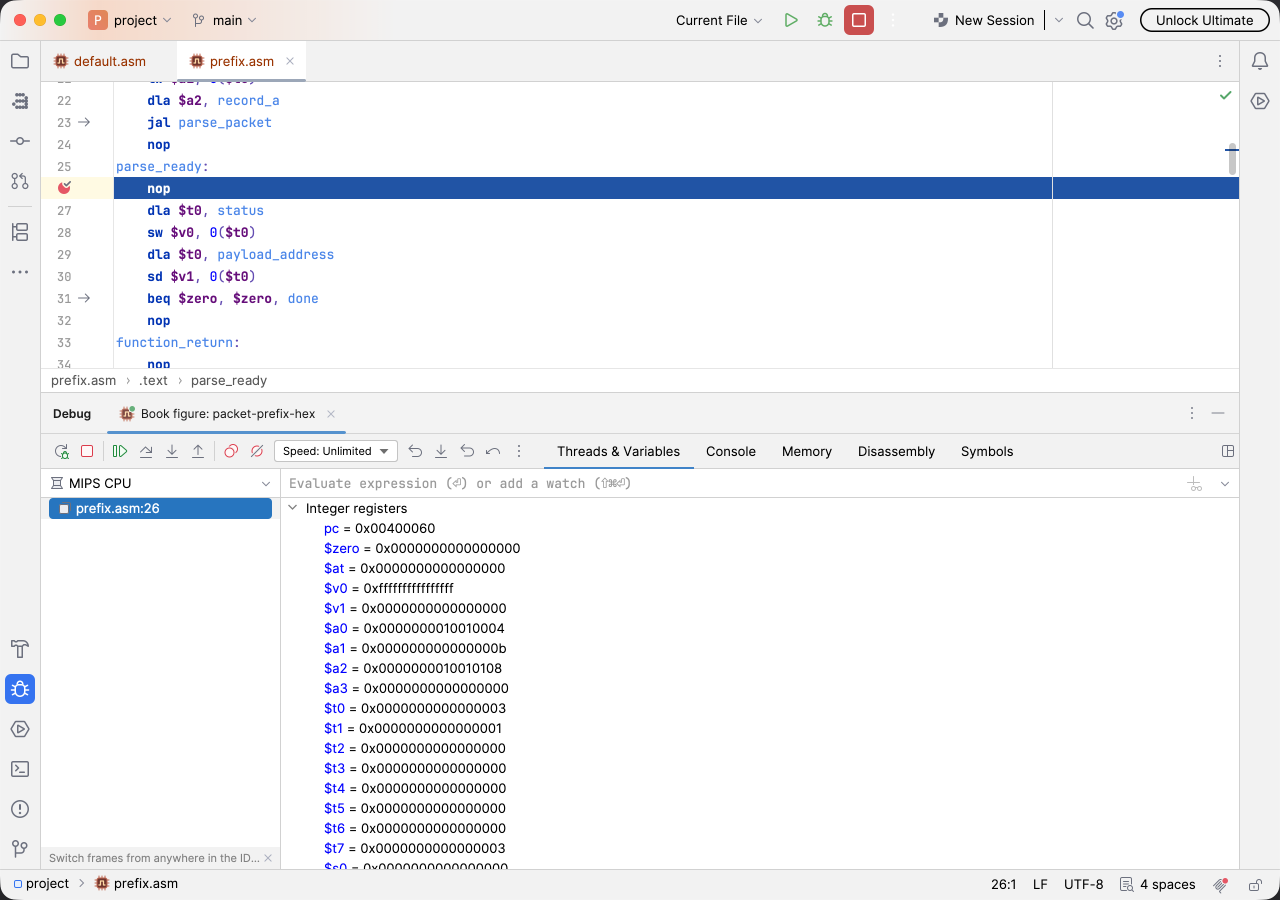
\includegraphics[width=0.54\linewidth,artifact,trim={\MARSpacketprefixsourceLeft{} \MARSpacketprefixsourceBottom{} \MARSpacketprefixsourceRight{} \MARSpacketprefixsourceTop{}},clip]{packages/013-binary-packet-parser/captures/f02-prefix/hex.png}};
    \begin{scope}[shift={(source.south west)},x={($(source.south east)-(source.south west)$)},y={($(source.north west)-(source.south west)$)}]
      \draw[black,line width=0.7pt] (0.215625000,0.057142857) rectangle (0.384375000,0.371428571);
      \node[draw=black,fill=white,circle,inner sep=1.5pt,font=\footnotesize] at ($(0.215625000,0.371428571)+(-3mm,0)$) {1};
    \end{scope}
    \node[anchor=north west,inner sep=0,font=\small\bfseries] (hex-title) at ([yshift=-3mm]source.south west) {Hexadecimal registers};
    \node[anchor=north west,inner sep=0] (hex) at ([yshift=-1mm]hex-title.south west) {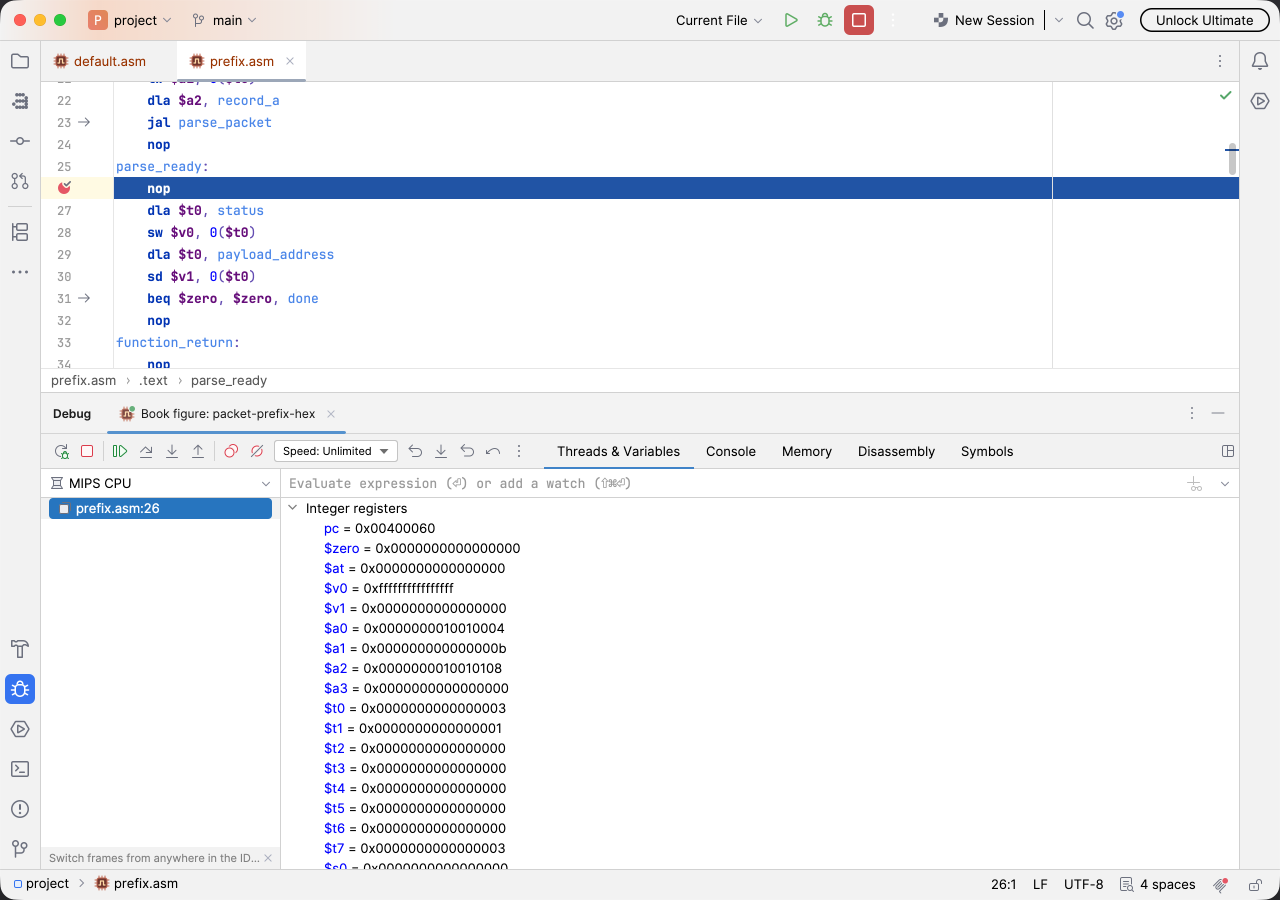
\includegraphics[width=0.42\linewidth,artifact,trim={\MARSpacketprefixhexLeft{} \MARSpacketprefixhexBottom{} \MARSpacketprefixhexRight{} \MARSpacketprefixhexTop{}},clip]{packages/013-binary-packet-parser/captures/f02-prefix/hex.png}};
    \begin{scope}[shift={(hex.south west)},x={($(hex.south east)-(hex.south west)$)},y={($(hex.north west)-(hex.south west)$)}]
      \draw[black,line width=0.7pt] (0.023437500,0.009708738) rectangle (0.753906250,0.980582524);
      \node[draw=black,fill=white,circle,inner sep=1.5pt,font=\footnotesize] at ($(0.023437500,0.980582524)+(-3mm,0)$) {2};
    \end{scope}
    \node[anchor=north west,inner sep=0,font=\small\bfseries] (decimal-title) at (0.58\linewidth,0 |- hex-title.north) {Signed return values};
    \node[anchor=north west,inner sep=0] (decimal) at ([yshift=-1mm]decimal-title.south west) {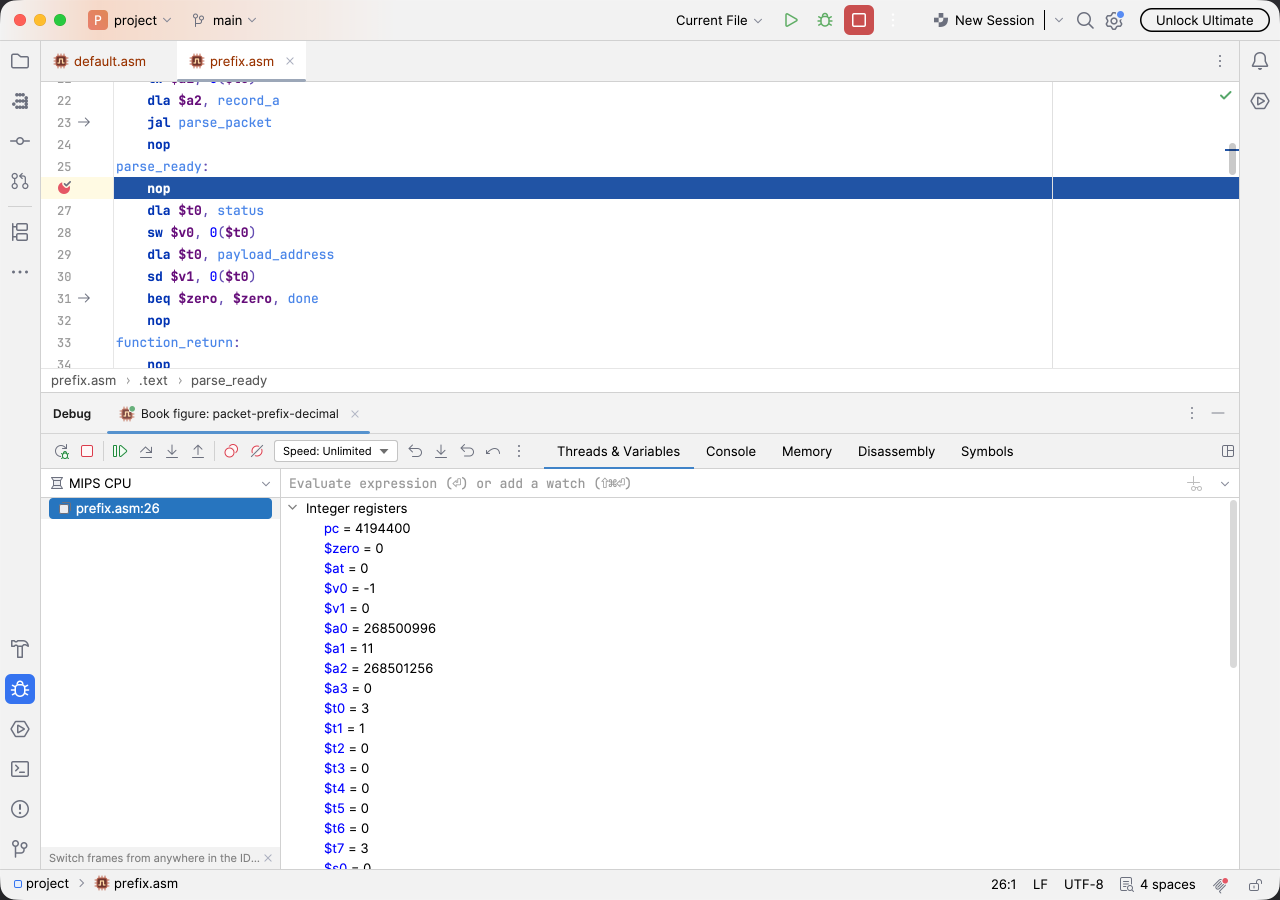
\includegraphics[width=0.42\linewidth,artifact,trim={\MARSpacketprefixdecimalLeft{} \MARSpacketprefixdecimalBottom{} \MARSpacketprefixdecimalRight{} \MARSpacketprefixdecimalTop{}},clip]{packages/013-binary-packet-parser/captures/f02-prefix/decimal.png}};
    \begin{scope}[shift={(decimal.south west)},x={($(decimal.south east)-(decimal.south west)$)},y={($(decimal.north west)-(decimal.south west)$)}]
      \draw[black,line width=0.7pt] (0.023437500,0.023255814) rectangle (0.242187500,0.953488372);
      \node[draw=black,fill=white,circle,inner sep=1.5pt,font=\footnotesize] at ($(0.023437500,0.953488372)+(-3mm,0)$) {3};
    \end{scope}
    \node[anchor=north west,inner sep=0,font=\small\bfseries] (input-title) at ([yshift=-3mm]hex.south west) {Mapped input bytes, including the preceding guard};
    \node[anchor=north west,inner sep=0] (input) at ([yshift=-1mm]input-title.south west) {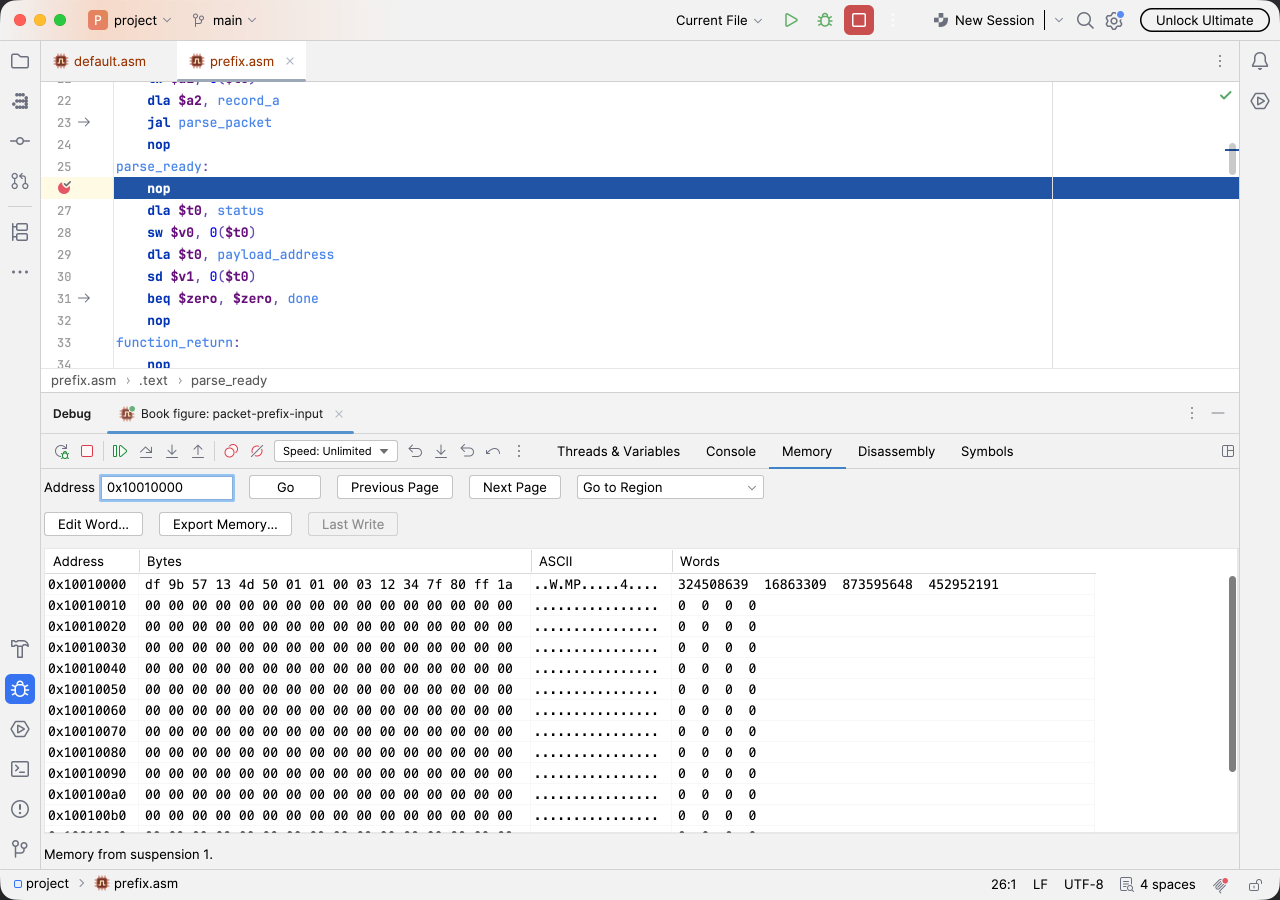
\includegraphics[width=0.84\linewidth,artifact,trim={\MARSpacketprefixinputLeft{} \MARSpacketprefixinputBottom{} \MARSpacketprefixinputRight{} \MARSpacketprefixinputTop{}},clip]{packages/013-binary-packet-parser/captures/f02-prefix/input.png}};
    \begin{scope}[shift={(input.south west)},x={($(input.south east)-(input.south west)$)},y={($(input.north west)-(input.south west)$)}]
      \draw[black,line width=0.7pt] (0.194672131,0.078431373) rectangle (0.997950820,0.490196078);
      \node[draw=black,fill=white,circle,inner sep=1.5pt,font=\footnotesize] at ($(0,0.490196078)+(-3mm,0)$) {4};
    \end{scope}
    \node[anchor=north west,inner sep=0,font=\small\bfseries] (record-title) at ([yshift=-3mm]input.south west) {Output record and its neighboring words};
    \node[anchor=north west,inner sep=0] (record) at ([yshift=-1mm]record-title.south west) {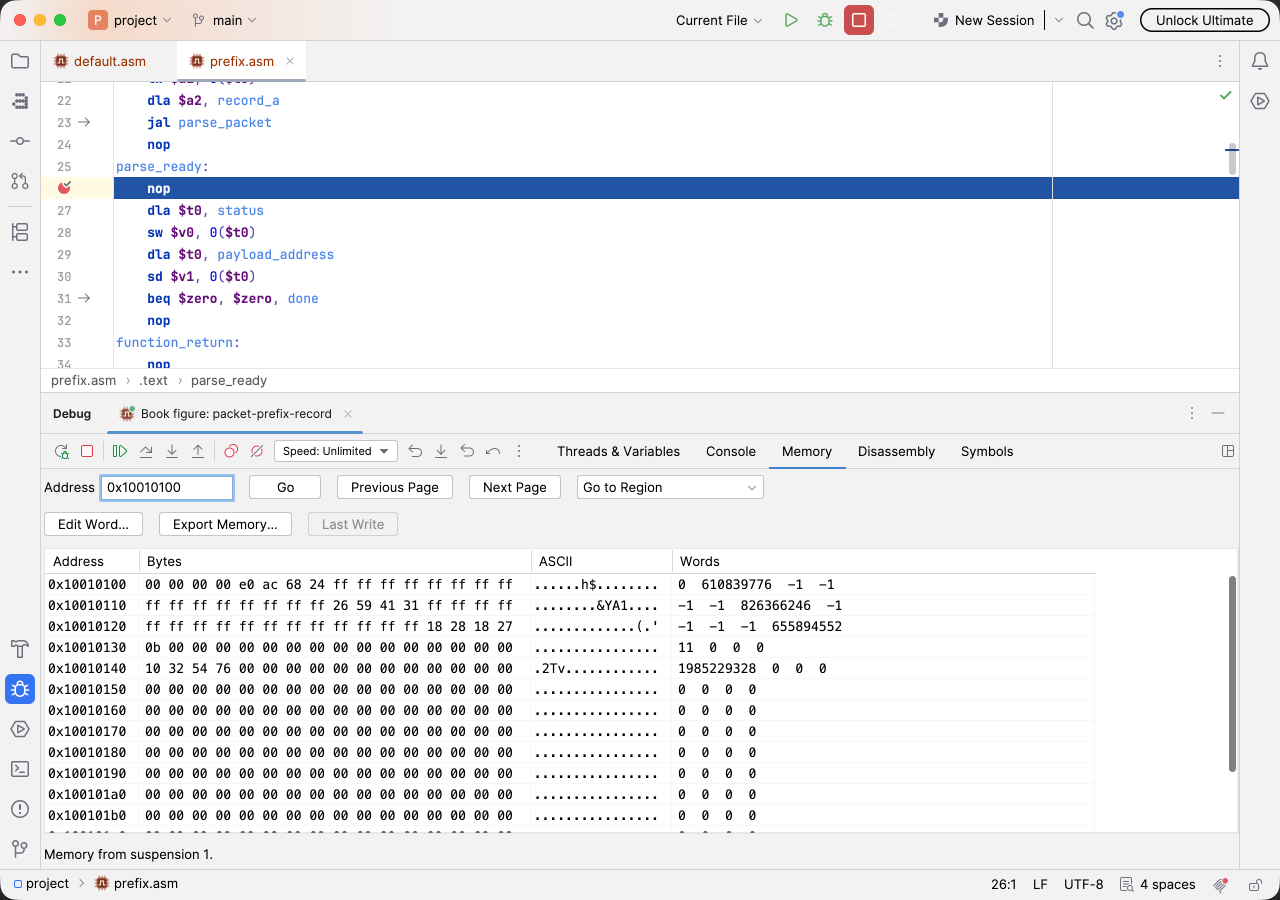
\includegraphics[width=0.84\linewidth,artifact,trim={\MARSpacketprefixrecordLeft{} \MARSpacketprefixrecordBottom{} \MARSpacketprefixrecordRight{} \MARSpacketprefixrecordTop{}},clip]{packages/013-binary-packet-parser/captures/f02-prefix/record.png}};
    \begin{scope}[shift={(record.south west)},x={($(record.south east)-(record.south west)$)},y={($(record.north west)-(record.south west)$)}]
      \draw[black,line width=0.7pt] (0.194672131,0.055555556) rectangle (0.997950820,0.638888889);
      \node[draw=black,fill=white,circle,inner sep=1.5pt,font=\footnotesize] at ($(0,0.638888889)+(-3mm,0)$) {5};
    \end{scope}
  \end{tikzpicture}
  \par\smallskip
  \begin{minipage}{\linewidth}
    \small
    \begin{enumerate}
      \setlength{\itemsep}{2pt}
            \setlength{\parsep}{0pt}
      \item This launch changes only \texttt{available} from 12 to 11. The same \texttt{parse\_ready} marker is next after the parser returns. The physical input allocation and all twelve packet bytes are unchanged.
      \item \texttt{\$a1 = 0x0b} means eleven available bytes beginning at \texttt{\$a0 = 0x10010004}. The result bits in \texttt{\$v0} are all ones; \texttt{\$v1} is zero. The output pointer in \texttt{\$a2} still names \texttt{record\_a}; it does not authorize an incomplete parse to write there.
      \item The native signed-decimal view reads \texttt{\$v0 = -1}: need more input. A null \texttt{\$v1} supplies no payload slice. The header declares three payload bytes, so completion requires $8+3+1=12$ bytes. Eleven available bytes are insufficient even though the payload itself is present.
      \item The admitted addresses end at \texttt{0x1001000e}, the payload byte \texttt{ff}. Trailer \texttt{1a} at \texttt{0x1001000f} remains mapped and visible, but lies outside that prefix. A debugger can display it without granting the parser permission to read it. The execution-read trace confirms that the parser does not inspect that trailer.
      \item At \texttt{0x10010108} through \texttt{0x10010117}, all four record words remain \texttt{0xffffffff}, or $-1$. The first two are at the end of the first line; the other two begin the next. The trace separately establishes zero record stores. Matching final bytes alone would not detect a temporary write followed by restoration.
    \end{enumerate}
  \end{minipage}
  \caption{Eleven available bytes exclude the checksum trailer even though it remains mapped and visible.}
  \label{capture:013-binary-packet-parser-f02-prefix}
  \label{packet-f02-prefix}
\end{figure}
\par
